\documentclass[kravspec/krav.tex]{subfiles}

\begin{document}

\section{Översikt av systemet}

\begin{figure}[h]
    \centering
    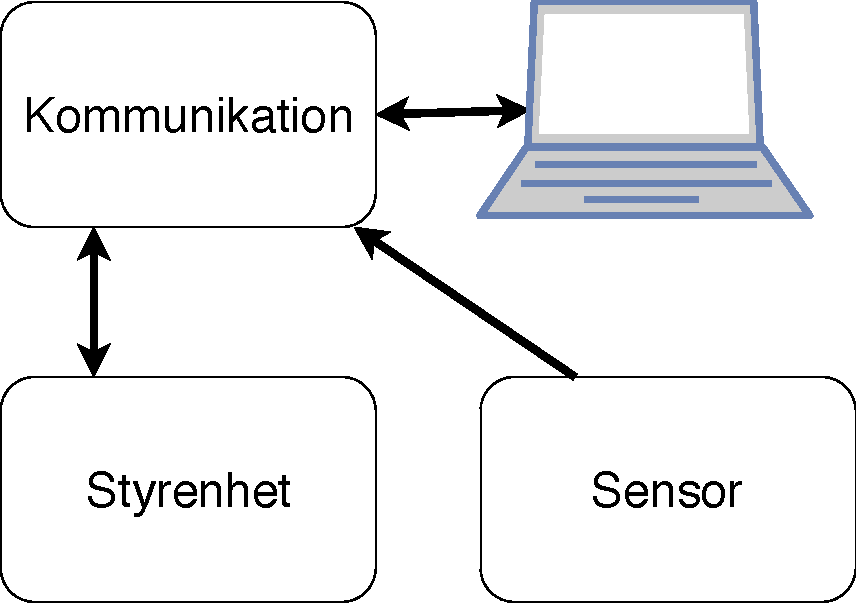
\includegraphics[width=0.6\linewidth]{kravspec/figures/overview-schema.pdf}
    \caption{Grov blockschema över moduler i produkten}
    \label{fig:overview}
\end{figure}

\subsection{Grov beskrivning av produkten}
Produkten är en bil med fyra hjul som ska med hjälp av ett känt vägnät ta sig
till en passagerare och skjutsa passageraren till önskad destination. Denna
taxibil ska kunna åka framåt, bakåt, svänga vänster och höger.  Bland annat ska
man kunna initiera en bluetooth-länk mellan bilen och en dator som har stöd för
bluetooth. Bilen ska ha ett läge där man kan fjärrstyra bilen och ett läge där
bilen ska köra autonomt i vägnätet samt undvika hinder.

\subsection{Produktkomponenter}
Lämplig hårdvara med kompletterande mjukvara kommer finnas i den kompletta
produkten. Bland annat ska även tekniskt dokumenation ingå i produkten.

\subsection{Beroenden till andra system}
Fjärstyrning av bilen skall vara beroende av en dator som har stöd för bluetooth.
Autonoma läget aktiveras från användargränsnittet tillgänglig på datorn med
bluetooth.

\subsection{Ingående delsystem}
En kommunikationsenhet, en styrmodul och en sensormodul enligt figur
\ref{fig:overview}. Sensormodulen ska hämta in data om omgivningen, bland annat
en kamera som tar bilder av vad som är framifrån, en sensor som mäter avstånd
till objekt i omgivning och tejpföljare som sensorer. Lämplig data av omgivning
skickas till kommunikationsmodell. Produkten har även en styrmodul som ser till
att bilen kan styras beroende på data från kommunikationsmodul.

\subsection{Avgränsningar}
Små väghinder som grova vägkanter och gropar tas ej hänsyn till. Vägen
förväntas bestå av hinder som är i lämplig höjd för att enhetens sensorer ska
upptäcka dem. Vägen antas vara plan utan gropar.

\subsection{Generella krav på hela systemet}

\begin{reqlist}
    \req{Taxin skicka aktuell mätdata till den bärbara datorn. Mätdata
    inkluderar avstånd till vägkant, avstånd till hinder, avlagd sträcka,
    styrbeslut och motorernas styrning}
    \req{Taxin skall via fjärrstyrning kunna köra framåt, bakåt och svänga
    vänster eller höger.}
    \req{Under autonom körning skall taxin navigera vägnätet enligt
    högertrafik.}
    \req{Under autonom körning skall taxin ej köra in i hinder.}
    \reqspec{original}{2}{Om ett hinder blockerar taxins körfält under autonom
    körning skall taxibilen köra runt objektet genom att köra i det andra
    körfältet.}
    \req{Under autonom körning skall taxin navigera genom vägnätet från en
    godtycklig position till en godtycklig given destination.}
    \reqspec{original}{3}{Bilen skall aktivera blinkers vid svängning samt
    hämtning och avlämning.}
\end{reqlist}

\end{document}
